% Source: graduate-coursework/Sp26/CSCE763/Course_Assignments/Exam/Midterm_Exam_solutions.tex

\documentclass[border=4pt]{standalone}
\usepackage{amsmath}
\usepackage{amssymb}
\usepackage{graphicx}
\usepackage{tikz}
\usepackage{xcolor}
\usetikzlibrary{shapes.geometric, arrows.meta, positioning, patterns, calc}

\definecolor{USC_Garnet}{HTML}{73000A}
\definecolor{USC_Sandstorm}{HTML}{FFF2E3}
\definecolor{USC_Black90}{HTML}{363636}
\definecolor{USC_Black70}{HTML}{5C5C5C}
\definecolor{USC_Black50}{HTML}{A2A2A2}
\definecolor{USC_Black10}{HTML}{ECECEC}
\definecolor{USC_Honeycomb}{HTML}{65780B}
\definecolor{USC_Atlantic}{HTML}{466A9F}
\definecolor{USC_Congaree}{HTML}{1F414D}
\definecolor{USC_Rose}{HTML}{CC2E40}

\newcommand{\problem}[1]{%
  \vspace{0.5cm}
  {\noindent\normalsize \textbf{#1}}
  \vspace{0.3cm}
}

\begin{document}
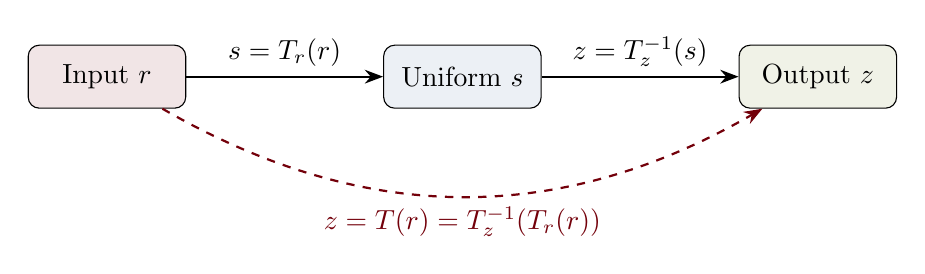
\begin{tikzpicture}[node distance=2.5cm, >=Stealth]
    \node (r) [draw, rounded corners, fill=USC_Garnet!10, minimum width=2cm, minimum height=0.8cm] {Input $r$};
    \node (s) [draw, rounded corners, fill=USC_Atlantic!10, minimum width=2cm, minimum height=0.8cm, right=of r] {Uniform $s$};
    \node (z) [draw, rounded corners, fill=USC_Honeycomb!10, minimum width=2cm, minimum height=0.8cm, right=of s] {Output $z$};

    \draw[->, thick] (r) -- node[above] {$s = T_r(r)$} (s);
    \draw[->, thick] (s) -- node[above] {$z = T_z^{-1}(s)$} (z);

    \draw[->, thick, USC_Garnet, dashed] (r) to[bend right=30] node[below] {$z = T(r) = T_z^{-1}(T_r(r))$} (z);
\end{tikzpicture}
\end{document}
